% journal of hydrology
% !TEX TS-program = pdflatex
% !TEX encoding = UTF-8 Unicode

% This is a simple template for a LaTeX document using the "article" class.
% See "book", "report", "letter" for other types of document.

\documentclass[11pt]{article} % use larger type; default would be 10pt

\usepackage[utf8]{inputenc} % set input encoding (not needed with XeLaTeX)

%%% Examples of Article customizations
% These packages are optional, depending whether you want the features they provide.
% See the LaTeX Companion or other references for full information.

%%% PAGE DIMENSIONS
\usepackage{geometry} % to change the page dimensions
\geometry{a4paper} % or letterpaper (US) or a5paper or....
% \geometry{margin=2in} % for example, change the margins to 2 inches all round
% \geometry{landscape} % set up the page for landscape
%   read geometry.pdf for detailed page layout information

\usepackage{graphicx} % support the \includegraphics command and options

% \usepackage[parfill]{parskip} % Activate to begin paragraphs with an empty line rather than an indent

%%% PACKAGES
\usepackage{url}
\usepackage{hyperref}
\usepackage{listings}
\usepackage{xcolor}
\usepackage{multirow}

\definecolor{codegreen}{rgb}{0,0.6,0}
\definecolor{codegray}{rgb}{0.5,0.5,0.5}
\definecolor{codepurple}{rgb}{0.58,0,0.82}
\definecolor{backcolour}{rgb}{0.95,0.95,0.92}

\usepackage{booktabs} % for much better looking tables
\usepackage{array} % for better arrays (eg matrices) in maths
\usepackage{paralist} % very flexible & customisable lists (eg. enumerate/itemize, etc.)
\usepackage{verbatim} % adds environment for commenting out blocks of text & 
%for better verbatim
%\usepackage{amsmath}
\usepackage{amsmath,amssymb}
\DeclareMathOperator{\E}{\mathbb{E}}

\usepackage{natbib}
\bibliographystyle{abbrvnat}
\setcitestyle{authoryear} %,open={((},close={))}}

\usepackage{subfigure}
%\usepackage{pageslts}

%\usepackage{subfig} % make it possible to include more than one captioned 
%%figure/table in a single float
% These packages are all incorporated in the memoir class to one degree or another...

%%% HEADERS & FOOTERS
\usepackage{fancyhdr} % This should be set AFTER setting up the page geometry
\pagestyle{fancy} % options: empty , plain , fancy
%\renewcommand{\headrulewidth}{0pt} % customise the layout...
%\lhead{}\chead{}\rhead{}
\lfoot{}\cfoot{\thepage}\rfoot{}
%\lfoot{}\cfoot{Page \thepage\ (\theCurrentPage) of 
%\lastpageref{LastPages}}\rfoot{}

%%% SECTION TITLE APPEARANCE
\usepackage{sectsty}
\allsectionsfont{\sffamily\mdseries\upshape} % (See the fntguide.pdf for font help)
% (This matches ConTeXt defaults)

%%% ToC (table of contents) APPEARANCE
\usepackage[nottoc,notlof,notlot]{tocbibind} % Put the bibliography in the ToC
\usepackage[titles,subfigure]{tocloft} % Alter the style of the Table of Contents
\renewcommand{\cftsecfont}{\rmfamily\mdseries\upshape}
\renewcommand{\cftsecpagefont}{\rmfamily\mdseries\upshape} % No bold!

%%% END Article customizations

%%% The "real" document content comes below...

\title{Final Report (Draft): \\
Image Analysis using Artificial Intelligence to
Quantify the Number and Density of Mussels in Lake Erie and Ontario}

\author{Angus Galloway}
%\date{} % Activate to display a given date or no date (if empty),
         % otherwise the current date is printed
         
\pagenumbering{roman}         

\lstdefinestyle{mystyle}{
    backgroundcolor=\color{backcolour},   
    commentstyle=\color{codegreen},
    keywordstyle=\color{magenta},
    numberstyle=\tiny\color{codegray},
    stringstyle=\color{codepurple},
    basicstyle=\ttfamily\footnotesize,
    breakatwhitespace=false,         
    breaklines=true,                 
    captionpos=b,                    
    keepspaces=true,                 
    numbers=left,                    
    numbersep=5pt,                  
    showspaces=false,                
    showstringspaces=false,
    showtabs=false,                  
    tabsize=2
}

\lstset{style=mystyle}

\begin{document}

\maketitle

\thispagestyle{empty}

\vspace{5cm}

\begin{centering}

Report prepared for:

\vspace{1cm}

Dominique Brunet \\ 
Environment Canada \\ 
867 Lakeshore Rd \\
Burlington, ON \\
L7S 1A1 

\end{centering}

\clearpage

% an introduction, a technical discussion of the steps taken, the rationale for
% the various design choices made and parameters selected for the training of
% the computer vision model, a technical discussion summarizing the
% strengths and limitations of the computer vision model and its robustness to 
% change to change of image resolution, viewing angle and other relevant
% factors, a discussion detailing how data acquisition methods can be improved
% in future surveys, and conclusions and include, as applicable, supporting
% graphs, tables and figures.

\setcounter{page}{1}

\section*{Executive Summary}
% 250 words or less

Measuring invasive mussel populations is essential to manage their impact on 
Great Lake ecosystems. Existing measurements are performed manually by divers 
that harvest mussels for a subsequent lab analysis. This process is expensive 
and difficult to scale throughout the Great Lakes, yielding incomplete data. 
Conversely, this proof-of-concept examines the use of artificial intelligence
(AI) to infer live coverage, biomass, and population, of in place mussels from
still images and video.

Qualitatively, the AI models identify both clusters as well as individual 
mussels on held out test cases, with relatively few false alarms. Further, 
models were found to generalize reasonably well to diverse underwater 
illuminations, seasonality, camera orientations and resolutions, as well as 
video, after training on only small patches extracted from 176 full size 
labeled images. 

Correlation between the predictions and lab measurements (e.g.~biomass, 
counts) for the underwater data is currently low, primarily due to occlusion 
from sediment and vegetation, empty shells, and some cases with low 
illumination. Only mussels that could be unambiguously identified were 
annotated as such. Agreement between the predictions and diver estimated live 
coverage is higher. For images taken in the lab, biomass and count were 
estimated reliably, with model predictions being more consistent than the
human-supplied segmentation labels. 

Results could be further improved by seeking additional labels from an online 
service at \$6.40 USD each. Image acquisition should ensure 
sufficient illumination; the camera to object distance relatively consistent;
vegetation removed, or that models are deployed during earlier months when algae
less present; empty shells similar in colour as live mussel removed, or treated
as ``mussel''. These changes will enable more 
accurate biomass and population counts in place.

\clearpage

\tableofcontents

\clearpage

\section*{Abbreviations}

\begin{description}
\item[API] application programming interface
\item[CE] Cross entropy
\item[CNN] convolutional neural network
\item[DL] deep learning
\item[DNN] deep neural network
\item[FCN] fully convolutional neural network
\item[IoU] intersection over union
\item[mIoU] mean IoU
\item[ML] machine learning
\item[SGD] stochastic gradient descent
\item[TP] true positive
\item[w.r.t.] with respect to
\end{description}

\clearpage

\pagenumbering{arabic}
\setcounter{page}{1}

\section{Introduction}

Measuring the density of invasive Zebra and Quagga mussels is essential to 
manage their adverse impacts on Great Lake ecosystems. Measurements are
currently performed manually by teams of divers that collect mussels
from a known area for analysis in a lab where they are subsequently freeze 
dried, weighed, and their diameter determined by sieve. This process is 
laborious, costly, and cannot be readily scaled up for mapping large areas 
throughout the Great Lakes. To this end, a proof-of-concept was 
devised to examine the feasibility of using artificial intelligence (AI) to 
infer live coverage, biomass, and mussel populations in place underwater 
solely from still images and video data.

The task of predicting mussel biomass, count, and percent coverage was cast as
that of~\emph{semantic segmentation} in machine learning. This means that a 
categorical prediction is assigned to each pixel in an image, where the
categories are associated to some~\emph{semantic} meaning, for example 
``pedestrian'', ``road'', or ``vehicle''. In general, the number of samples
required to learn to discriminate between $C$ classes with a fixed accuracy 
increases with $C$.\footnote{It follows from an information-theoretic analysis
of traditional classification that the sample complexity scales linearly with
$C$ at best, although the precise form of this relationship is not clear for 
semantic segmentation with deep neural networks.} The problem was therefore
formulated as a pixelwise binary classification between~\texttt{background} 
and~\texttt{mussle}. It is expected that the number of pixels output 
as~\texttt{mussle}, combined with the camera resolution, distance, and surface
area should be predictive of the mussel biomass and their count after 
further processing.

\section{Data Preparation}

It is known that~\emph{supervised} machine learning, and deep learning in 
particular, often relies on vast quantities of labeled samples from which to 
learn. Although 1,608 analyses with ground truth scalar measurements such as 
biomass have been provided, there are computational as well as 
information-theoretic challenges associated with attempting to learn directly 
from such a dataset. 
The computational challenge is that the typical image resolution used to train
state-of-the-art deep neural networks such that they do not exceed available
GPU memory is around 256 square pixels -- about an order of magnitude less than
the high image resolutions in the mussels dataset. 

The second challenge is that learning an end-to-end prediction on the basis of 
a scalar error, for example w.r.t.~biomass, has a low signal-to-noise 
ratio. Such an approach would require i) reducing the image resolution until
models fit in memory resulting in significant information loss, ii) yield
spurious correlations, for example between substrate type and count, as 
the actual task of~\emph{counting} mussel instances would not be solved, 
nor would sufficient detail be available to do so.

Fortunately, fully convolutional neural network (FCN) architectures gracefully 
scale to arbitrary image resolutions, and can thus be trained on batches 
comprised of smaller patches and tested on whole images. 

A training dataset was prepared using~\texttt{GLNI} data primarily collected in 
2017 and 2018. This data was attractive as a metal frame held the camera, thus
the quadrat to camera mapping was approximately fixed. Furthermore, a
consistent distance between the camera and substrate was believed to increase
the robustness of learned features to other sources of variation including 
seasonality, water colour, substrate type, and partial occlusions.

In many cases multiple images were captured for the same analysis and assigned 
a~\textbf{File \#}. Generally, the image with the highest suffix number was 
selected for inclusion in the dataset, which greatly reduced the number 
of candidates for labeling (e.g.~from 403 to 179 for the 
2019~\texttt{GLNI} data). 

The quadrat interior was extracted resulting in a 3000 square pixel image,  
which was scaled by $75\%$ with interpolation using OpenCV. The resulting 2250
square pixel image -- the ``originals'' -- were either labeled manually by the 
consultant or using paid crowd-sourcing methods. Pairs of original and labeled
image were then cropped to $250 \times 250$ pixel patches, depicted in
Figure~\ref{fig:original-to-patch}. 

The training set (\texttt{train\_v111}) contains 121 originals and 9,801 
patches, while the 2019 GLNI validation set (\texttt{val\_v101}) contains 55 
originals and 4,455 patches. For model deployment and assessment of 
generalization to non-GLNI data, for example Tripod and WHERD, it is 
recommended to train on both splits (\texttt{trainval\_v111}) for 14,256 total 
patches. 
This is competitive with the PASCAL Visual Object Classes (VOC) Challenge 
dataset, which has become a standard benchmark for semantic segmentation 
models, is of a similar resolution and contains 6,929 ground truth 
segmentations but 20 object classes~\citep{everingham2015pascal}. As such, it
is anticipated that publication of this dataset may be of independent interest 
to the machine learning and computer vision communities.

\begin{figure}
\centering
\subfigure[]{
\includegraphics[width=0.44\linewidth]{./img/GLNI_12-2_2019-07-25_image-1_crop_img_viz.jpg}
\label{sub:original-img-to-patch}}
\subfigure[]{
\includegraphics[width=0.44\linewidth]{./img/GLNI_12-2_2019-07-25_image-1_crop_lab_viz.png}
\label{sub:original-lab-to-patch}}
\caption{Extraction of $250 \times 250$ pixel patches from an 
original input~\subref{sub:original-img-to-patch} and its ground truth
segmentation~\subref{sub:original-lab-to-patch}. This step yields 81 training 
images per sample and provides a sense of the spatial context of the
predictions.}
\label{fig:original-to-patch}
\end{figure}

\subsection{Sourcing Ground Truth Labels}

This section describes the usage of three sources of ground truth semantic 
segmentation labels. A detailed comparison of the three labeling methods is 
provided in Table~\ref{tab:label-services}.

\begin{enumerate}
\item~\texttt{LabelMe}
was initially developed as an online tool by 
the MIT Computer Science and Artificial Intelligence Laboratory
(CSAIL)~\citep{russell2008labelme}. Since then, high quality open source 
desktop 
versions have been implemented in Python and the popular Qt graphics 
library\footnote{Tool available for download at this 
URL~\url{https://github.com/wkentaro/labelme}}. Slightly more than
$50\%$ of the 233 originals that were labeled from scratch or modified during 
the project were done by the consultant using this tool. The tool accepts 
images in either jpeg or png format and outputs a~\texttt{json} file with the 
same name as each image upon saving the annotation. The mean time to label an 
original image from scratch was around 5-15 minutes, with some images with 
hundreds of mussels taking 45 minutes.

\item~\texttt{Figure Eight}~(\url{https://figure-eight.com/}:\footnote{formerly
``CrowdFlower''}, is a human-in-the-loop data annotation company, and services 
large enterprises like Google and Facebook. A labeling interface and set of
instructions to be shown to workers was designed via a graphical online 
interface and with some coding of environment variables. Several days were
spent tuning the design of the task interface shown to workers and configuring 
automated quality control tests before results of moderate quality were 
returned. Overall the system required a high degree of supervision to ensure
the responses were appropriate and that workers did not cheat. Additional 
details including the final configuration are provided in 
Appendix~\ref{sec:figure-eight}.

Before a total of 46 images from the Aug.~2017 subset of the training set were
deemed to be of sufficient quality for incorporation in the dataset, they had 
to be adjusted and missing mussels added using the~\texttt{LabelMe} tool. To do 
so, the 
notebook~\href{https://github.com/AngusG/cciw-zebra-mussel/blob/master/labelme/figure-eight/postprocess-figure-eight-labels.ipynb}{postprocess-figure-eight-labels.ipynb}
was used to convert the polygon vertices returned by~\texttt{Figure Eight} 
in~\texttt{json} format into that used by~\texttt{LabelMe}.

\item~\texttt{Scale AI}~(\url{https://scale.com/})

Unlike LabelMe and FigureEight, the Scale service is more of a black-box in 
which the user submits query images via an API in their preferred programming
language -- see source code Listing~\ref{lst:scale} for a minimal working 
Python example -- and a response is received within 4 to 48 hours in most 
cases. Rather than having to design a user interface, labeling instructions are 
provided as a text string argument to the API call. Upon receiving the 
response, users can audit the results via their website and view transparent 
labels imposed on the input image. In total 59 images were labeled by this 
service. Most labels were of high quality and could be used as-is, while a 
small number were adapted using the free GNU Image Manipulation Program (GIMP) 
with the procedure outlined in Appendix~\ref{sec:gimp}.

\end{enumerate}

Given the high quality, transparent pricing scheme and ability to handle
arbitrary volumes, as well as the autonomy and expediency with which results 
are returned, it is recommended to use the Scale service for all future 
labeling needs until volumes exceed 1000 images, after which point volume 
discounts or a custom solution should be considered.

\begin{table}[]
\centering
\caption{A comparison of three image labeling services for generating ground
truth semantic segmentation masks for mussel images:
\texttt{LabelMe},~\texttt{Figure Eight}, and~\texttt{Scale AI}.
Analysis done assuming two ($C=2$) classes ``mussel'' and ``background'', but
is expected to remain consistent for $C \leq 20$. Row F) ``Latency'' means the
time elapsed between when a label is requested for a particular image and the
time it is delivered, whereas G) ``Throughput'' refers to the number of images
processed per unit time (parallelism, i.e., many workers, increases
throughput). Clarifications: row J) Yes$^*$: User is responsible
for the creation of test examples that automatically reject low quality
judgments, otherwise the user must manually reject them. Rejected judgments 
incur the same fee as accepted judgments. Row M) Slack$^*$: Questions about 
volume discounts and re-submitting labels rejected during audit were 
acknowledged 02-28-2020 but remain unanswered.}
\begin{tabular}{lccc}
\toprule
Service & Manual (\texttt{LabelMe}) & \texttt{Figure Eight} & \texttt{Scale AI} 
\\ \midrule
A) Interface type & Desktop GUI & Web Interface & API \\ \midrule
B) Overhead complexity \\ (Amazon MTurk = 10) & 2 & 5 & 1 \\ \midrule
C) Trial mode duration \\ (in images labeled) & NA & 1000 (Paid) & 5 (Free) \\ 
\midrule
D) Minimum fee after trial & NA & 10,000 USD & NA \\ \midrule
E) Cost per image (USD) & -- & 2.25 & 6.40$^*$ \\ \midrule
F) Latency (m=min, h=hour) & $<60$m & $<60$m & $4-48$h \\ \midrule
G) Throughput & Low & High & High \\ \midrule
H) Quality & High & Medium--Low & High \\ \midrule
I) Guaranteed label for \\ all pixels & No & No & Yes \\ \midrule
J) User responsible for \\ quality assurance (QA) & Yes & Yes$^*$ & No \\  
\midrule
K) Edit labels in~\texttt{LabelMe} & Yes & Yes & No \\ \midrule
L) Edit labels in~\texttt{GIMP} & Yes & Yes & Yes \\ \midrule
M) User support & None & Email, Video Call & Slack$^*$ \\ \midrule
N) Images labeled & 126 & 64 & 59 \\ \bottomrule
\end{tabular}
\label{tab:label-services}
\end{table}

\subsection{Data Analysis}

Each of th $N=121$ original images which form the training set are
associated with a lab measurements and visually estimated live coverage. 
The analysis shown in Figure~\ref{fig:data-analysis} suggests that live
coverage is a poor predictor of biomass and count, however, biomass predicts 
the live coverage with $R^2 = 0.4090$. These results serve as a reference for 
the machine learning based predictions, which like the human diver, relies 
solely on visual cues to infer biomass and population count.

\begin{figure}
\centering
\subfigure[]{
\includegraphics[width=0.9\linewidth]{img/train_v111_predict_biomass_and_count_from_live_coverage.eps}
\label{fig:bio-ct-fr-cov}}
\subfigure[]{
\includegraphics[width=0.9\linewidth]{img/train_v111_predict_live_coverage_from_biomass_and_count.eps}
\label{fig:cov-fr-bio-ct}}
\caption{Plotting~\subref{fig:bio-ct-fr-cov} mussel biomass and count versus 
live coverage estimated by diver, and~\subref{fig:cov-fr-bio-ct} vice versa, 
for GLNI training data ($N=121$). Note that the $R^2$ coefficient of 
determination varies between the two rows since it is not symmetric.}
\label{fig:data-analysis}
\end{figure}



\section{Machine Learning Methodology}

The practice of machine learning involves the selection, or search for ``good'' 
meta-parameters. The prefix ``meta'' is used to distinguish the parameters of
the learning algorithm -- generally set by the practitioner -- from those of the
model, which are to be learned.\footnote{Meta-parameters are often called
hyper-parameters, but the latter term is reserved for parameters of 
probability distributions.}

Relevant meta-parameters include the step size or ``learning rate'' of gradient
descent (GD), and the mini-batch size, which is what distinguishes stochastic
gradient descent (SGD) from full-batch GD. 

Optional meta-parameters include L2 regularization, aka ``weight decay'',
which penalizes the squared $\ell_2$-norm of all parameters of the model.

Denote the neural network parameters at time step $t$ by $\theta_t$. The update
equation which determines the parameters at the next time step, $\theta_{t + 
1}$, is then:

\begin{equation} \label{eq:sgd}
\theta_{t + 1} = \theta_t + \eta \nabla_{\theta} \mathop{\mathbb{E}}_{x,y \sim 
X, Y} \big[ \mathcal{L}(y, \hat{y}) \big]
\end{equation}

The loss function $\mathcal{L}$ has as its arguments the input $x$, ground
truth labels $y$, and model predictions $\hat{y}$. Assume access to a dataset 
of $N$ samples (technically a sequence not a set) of pairs 
$\{ (x_i, y_i)\}_{i=1}^{N} $.

\subsection{Learning Rate Selection}

The learning rate, $\eta$ in Eq.~\eqref{eq:sgd}, controls the magnitude of the 
updates to the parameters at each update step. There is significant theory on
the optimal selection of learning rates in the case where the loss is a convex
function of the parameters, but less so when the loss is non-convex w.r.t.~the
parameters, as is the case in deep learning. Here, researchers often perform
simulations to determine the best learning rate on the basis of validation 
accuracy.

Nevertheless, some general comments can be made on the topic of learning rate 
selection in DL: 

\begin{enumerate}
\item a larger learning rate generally reduces the loss more quickly than a
smaller learning rate allowing one to see results more quickly, but, \dots
\item a larger learning rate may make training unstable
\item a larger learning rate -- for a fixed mini-batch size -- can be said to
be noisier than a smaller learning rate. Such noise tends to be helpful for 
promoting generalization, e.g., wide minima argument, however if the gradient 
is too noisy then the gradient signal-to-noise ratio may be too low thus 
slowing learning.
\item on the regularization effect of large initial learning rate.
\end{enumerate}

\subsection{Mini-Batch Size Selection}

Generally, there is a strong interplay between the batch size and the learning
rate. For training efficiency, one generally prefers the largest batch size
without overflowing available GPU memory.

Too large a batch size behaves similarly as too small a learning rate, thus may 
converge to a ``sharper'' minimum of the loss landscape. Conversely, too small 
a batch and the variance of the expectation in Eq.~\eqref{eq:sgd} will be too 
high.

\subsection{Segmentation Model Architectures}

Several segmentation architectures based on deep neural networks were
considered: 

\begin{description}
\item[FCN] Fully convolutional networks (FCN) were proposed 
by~\cite{long2015fully} \dots

\item[U-Net] Was originally proposed by~\cite{ronneberger2015unet} for 
biomedical image segmentation, where sharp edge boundaries, for example between 
affected and unaffected skin lessions are important. This architecture has 
since been successfully applied in many natural image domains unrelated to 
medical imaging. 
The model takes its name from its ``U'' shaped network diagram whereby the
input is encoded into a progressively smaller representation which reaches a 
bottleneck at the bottom of the ``U'', which is then gradually upsampled to the 
original image size while features from earlier encodings are concatenated to 
the decoded representations at each layer for spatial consistency.

\item[DeepLab] desc

\item[CRF] The conditional random field~\cite{krahenbuhl2011efficient} is not
itself a segmentation architecture, but a graphical model that is commonly used
for~\emph{structured prediction} tasks, and post-processing segmentation
predictions in particular.

\end{description}

\subsection{Evaluation Criteria}

Semantic segmentation performance is generally assessed in terms of the
intersection between predictions and the ground truth segmentation mask -- the
true positives -- divided by the union of the predictions and the ground truth, 
which includes both false negatives and false positives. This quantity is
referred to as the intersection-over-union (IoU), or mIoU after taking the
mean over samples in a dataset. This metric addresses a limitation of reporting 
pixelwise accuracy, since most datasets are dominated by background pixels,
thus a high accuracy could be obtained by a constant classifier that simply
predicts ``background''. Conversely, the binary IoU is formally defined as:

\begin{equation}
\frac{TP}{FN + TP + FP}
\end{equation}

Despite its widespread use, the binary mIoU metric has some limitations:

\begin{enumerate}
\item If legitimate images contain~\emph{none} of the foreground classes, i.e.,
the true label is $100\%$ background, the numerator ``TP'' is undefined and an
IoU score of 0 is assigned to a ``true negative'' prediction.

\item If the foreground pixel area varies significantly, IoU 
scores may be less comparable between images. For example, an image with $1\%$
\texttt{mussel} pixels in which $90\%$ are predicted correctly would be assigned
an equal weight w.r.t.~the sample mean as an image with $50\%$~\texttt{mussel}
of which only $50\%$ are identified as such. In this scenario, the sample with
$1\%$~\texttt{mussel} inflates the mIoU score.
\end{enumerate}

In light of these limitations, several variants of mIoU have been proposed to 
incorporate various weighting schemes.

\subsection{Data Augmentation and Pre-Processing}

\begin{enumerate}

\item Randomly flip images horizontally and vertically.

\item Normalize pixels from [0, 1] to [-1, 1].

\end{enumerate}

\section{Experiments}

The underwater dataset is referred to as ``In-Situ''.

\subsection{Biomass Prediction from Ground Truth Segmentation}

In this section we assess the quality of the obtained segmentation labels and
characterize the noise inherent in relating the mussel biomass to those mussels
identifiable by human eye.

\begin{figure}
\centering
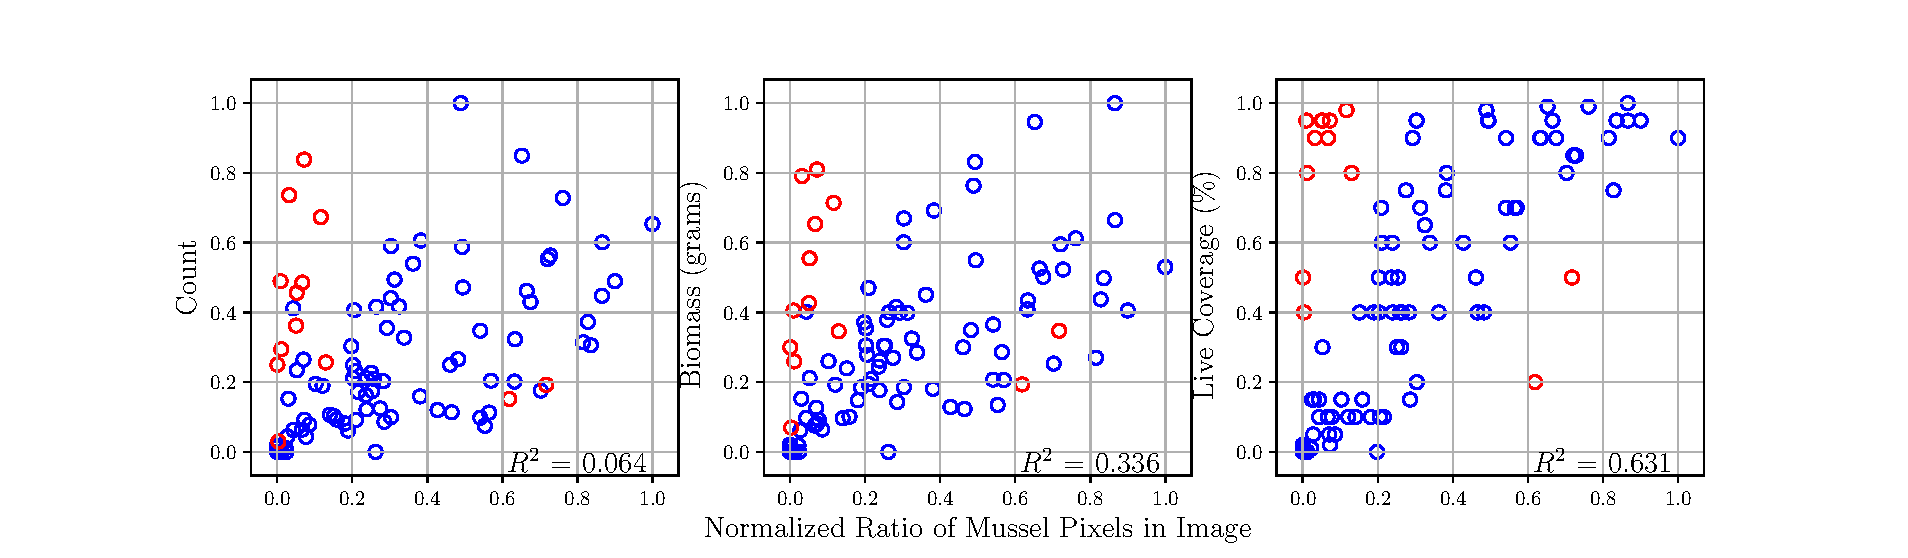
\includegraphics[width=0.9\linewidth]{img/Train-all-109-annotate-outliers}
\caption{Relationship between mussel count, biomass, and diver estimated live
mussel coverage versus pixels assigned to mussel class in ground truth
segmentation labels for GLNI training data ($N=109$). Note that because only 
those mussels that could be clearly identified as such were labeled, an upper 
triangular effect is observed where some images have few labeled mussels, 
but high biomass (e.g., due to occlusion from~\emph{Cladophora}). Removing 9 
such outliers (shown in red) increases the $R^2$ value three fold from $\approx
0.2$ to $0.63$. All ``outliers'' were intentionally under labeled due to
considerable occlusion by Cladophora, or a lack of illumination.}
\label{fig:train-biomass-from-labels}
\end{figure}


\subsection{Underwater Dataset}

plot showing IoU along with CE loss.

Model trained on~\texttt{val\_v101} set and evaluated on~\texttt{2018-06}
subset labeled by Scale.

\begin{table}[]
\caption{Confusion matrix for model trained on~\texttt{val\_v101} set and
evaluated on~\texttt{2018-06}.}
\centering
\begin{tabular}{llcc}
\toprule
\multicolumn{1}{c}{\multirow{2}{*}{Label}} & \multicolumn{1}{c}{1} & 0.26 & 
0.09 \\ \cmidrule{2-4}
\multicolumn{1}{c}{} & \multicolumn{1}{c}{0} & 0.19 & 0.46 \\ \cmidrule{2-4}
 &  & 1 & 0 \\
 &  & \multicolumn{2}{c}{Prediction} \\ \bottomrule
\end{tabular}
\end{table}

\begin{figure}
\centering
\subfigure[]{
\includegraphics[width=0.45\linewidth]{./img/GLNI_2909-1_2018-06-28_image-1_crop.jpg}
\label{sub:iou-i-1}}
\subfigure[]{
\includegraphics[width=0.45\linewidth]{./img/GLNI_2909-1_2018-06-28_image-1_crop__fcn8s_lr1e-03_wd5e-04_bs25_ep80_seed4_epoch70__TP66638_FP29221_FN540291_IoU0p1048.eps}
\label{sub:iou-p-1}}
\subfigure[]{
\includegraphics[width=0.45\linewidth]{./img/GLNI_3796-2_2018-06-26_image-3_crop.jpg}
\label{sub:iou-i-2}}
\subfigure[]{
\includegraphics[width=0.45\linewidth]{./img/GLNI_3796-2_2018-06-26_image-3_crop__fcn8s_lr1e-03_wd5e-04_bs25_ep80_seed4_epoch70__TP2199076_FP479652_FN184805_IoU0p7680.eps}
\label{sub:iou-p-2}}
\caption{Visualization of intersection-over-union (IoU) calculation for a 
sample with a low IoU value [\subref{sub:iou-i-1}-\subref{sub:iou-p-1}] and 
high IoU value [\subref{sub:iou-i-2}-\subref{sub:iou-p-2}]. 
For~\subref{sub:iou-p-1}: true positives (TP) = 66,638, false positives (FP) =
29,221, false negatives (FN) = 540,291, and IoU = 0.1015. 
For~\subref{sub:iou-p-2}: TP = 2,199,076, FP = 479,652, FN = 184,805, and IoU = 
0.7680. Samples from a held out the~\texttt{2018-06} split labeled by Scale and
model trained on~\texttt{val\_v101} split. Note that high FN 
in~\subref{sub:iou-p-1} may be due to under-labeling tendencies.}
\label{fig:iou-example}
\end{figure}


\subsection{Lab Dataset}

See Figure~\ref{fig:lab-to-lab-biomass-from-pixels}.

\newcommand{\labtolab}{./img/lab_to_lab/}

\begin{figure}
\centering
\subfigure[]{
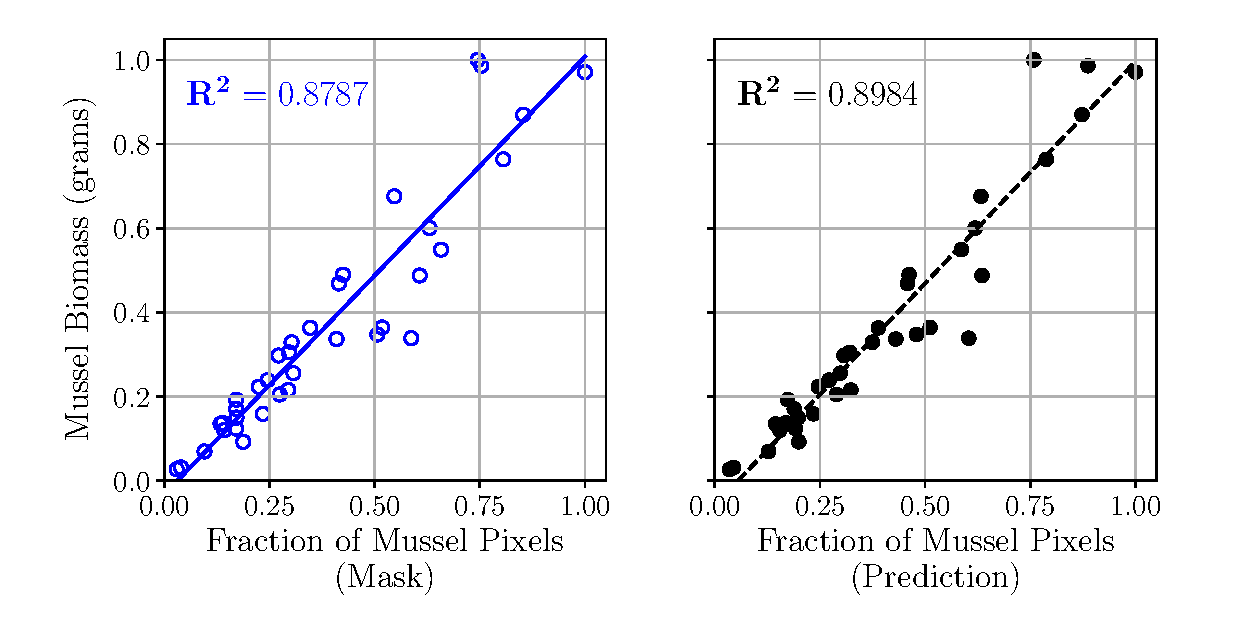
\includegraphics[width=0.9\linewidth]{\labtolab/lab_predict_biomass_from_pixels_no_cameraval_100-val_100__fcn8slim_lr1e-03_wd5e-04_bs32_ep50_seed1_epoch40.eps}
\label{sub:lab-biomass-default}}
\subfigure[]{
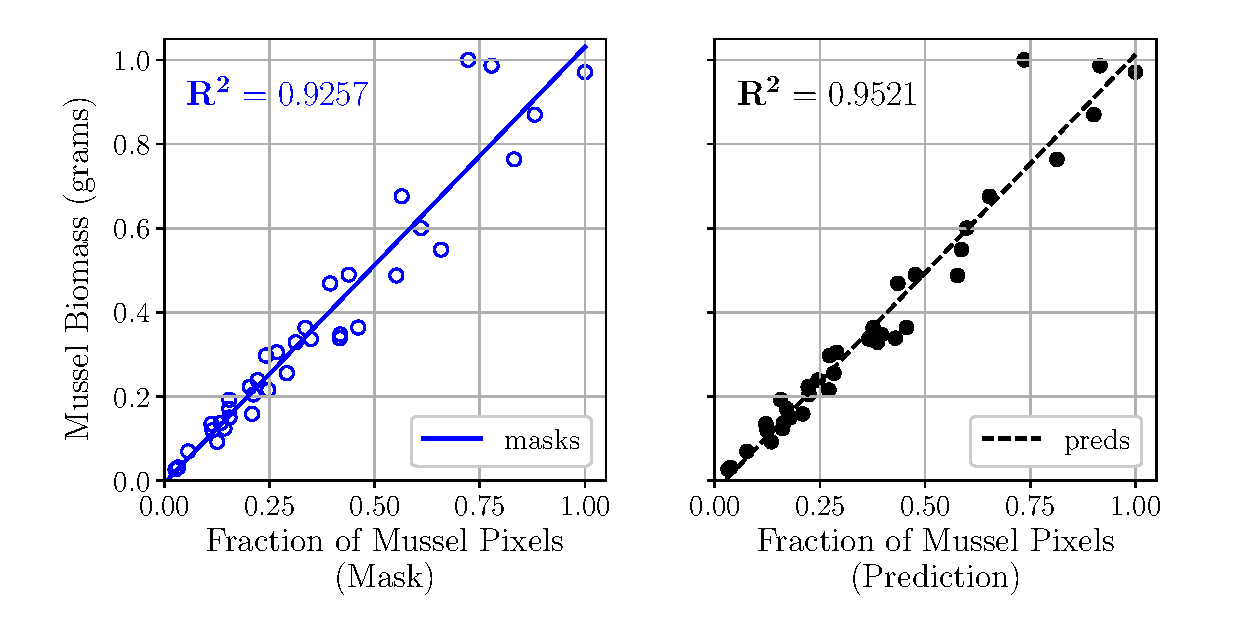
\includegraphics[width=0.9\linewidth]{\labtolab/lab_predict_biomass_from_pixelsval_100-val_100__fcn8slim_lr1e-03_wd5e-04_bs32_ep50_seed1_epoch40.eps}
\label{sub:lab-biomass-camera}}
\caption{Relationship between mussel biomass in grams and fraction of pixels in 
image mask (left column) or prediction (right column) assigned to mussel class.
Plot~\subref{sub:lab-biomass-default} is based on raw pixel count in images, 
while~\subref{sub:lab-biomass-camera} adjusts the number of pixels by the
product of the vertical and horizontal squares in the frame divided by the 
total number of squares ($16 \times 25$). The $R^2$ score, or proportion of
variance in biomass accounted for by mussel pixels is annotated in each plot.}
\label{fig:lab-to-lab-biomass-from-pixels}
\end{figure}

\begin{figure}
\centering
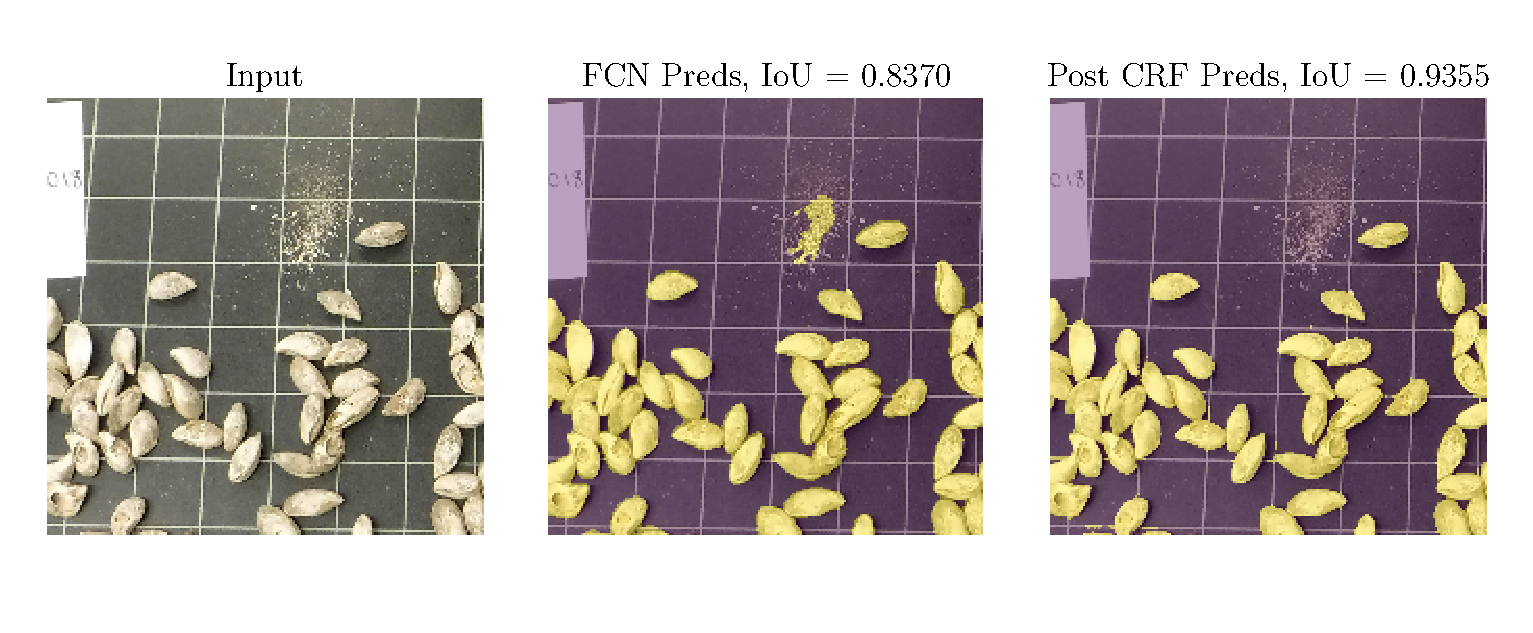
\includegraphics[width=0.9\linewidth]{\labtolab/val_100-val_100__Lab_3796-1_2018-08-13_image-1_patch_width1000_crf__fcn8slim_lr1e-03_wd5e-04_bs32_ep50_seed1_epoch40.eps}
\caption{Sample image patch and predictions with IoU score. Post processing 
by CRF improves IoU by 10\% absolute, primarily by eliminating the FP
predictions associated with the debris.}
\label{fig:lab-to-lab-sample}
\end{figure}


\subsection{Generalization From Underwater to Lab Dataset}

Figure~\ref{fig:zero-shot-situ-lab} shows model predictions that arise from
training on underwater data and evaluated on an unseen distribution of Lab
images. The generalization problem is difficult because mussels tend to sit in a
vertical orientation in the wild, with the dark gap between the two shell
halves acting as a primary visual basis for identification by human eye. 
Further, mussels tend to be darker underwater due to reduced illumination, or
from being covered with a fine layer of sediment. Conversely, Lab images are 
well illuminated and all mussels lie on their side. 

These qualitative differences between the two distributions are 
reflected in Figure~\ref{fig:zero-shot-situ-lab}. It appears that the brighter 
mussels -- which have a similar white colour as the unlabeled empty shells
underwater -- are the most prominent false positives, while the darker more 
textured area of the mussle shells are identified correctly.

\newcommand{\zshot}{./img/situ_to_lab/}

\begin{figure}
\centering
\subfigure{
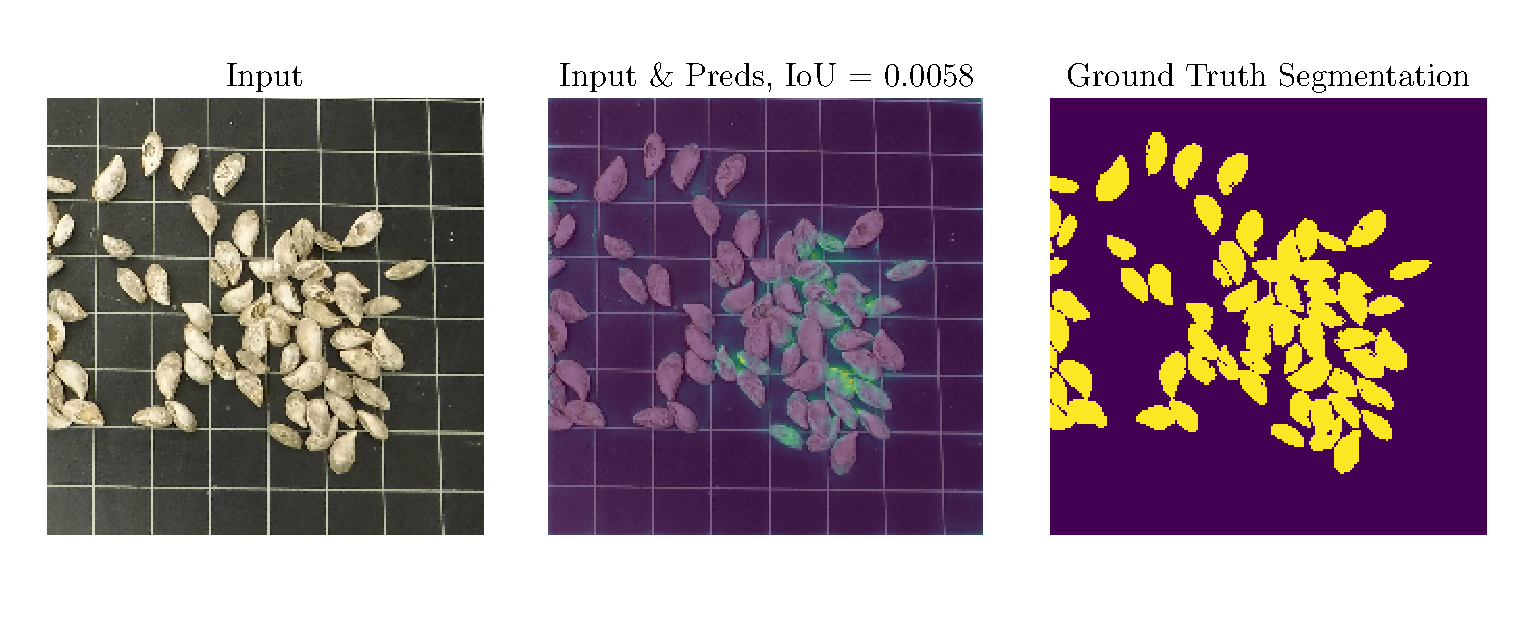
\includegraphics[width=0.9\linewidth]{\zshot/val_101-lab_100__Lab_3796-1_2018-08-13_image-1_patch_width1200__fcn8s_lr1e-03_wd5e-04_bs25_ep80_seed4_epoch70.eps}}
\subfigure{
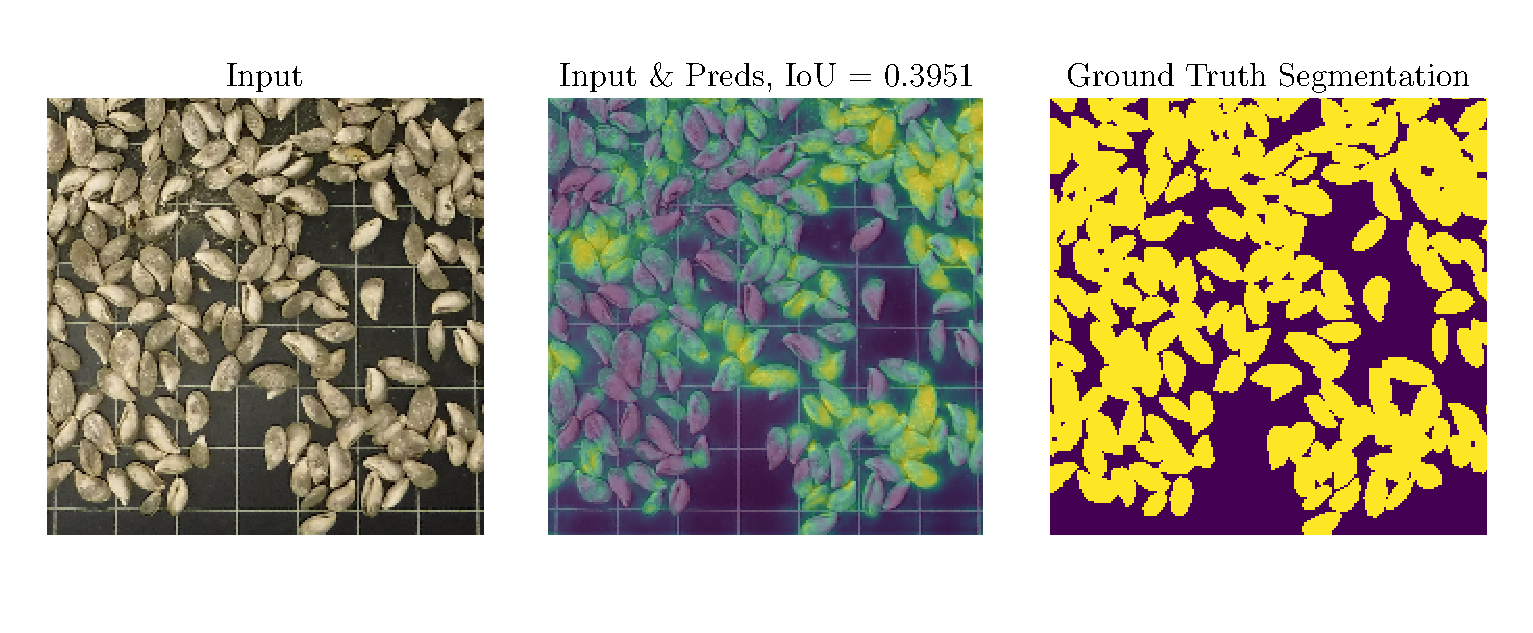
\includegraphics[width=0.9\linewidth]{\zshot/val_101-lab_100__Lab_3798-2_2018-08-13_image-1_patch_width1200__fcn8s_lr1e-03_wd5e-04_bs25_ep80_seed4_epoch70.eps}}
\subfigure{
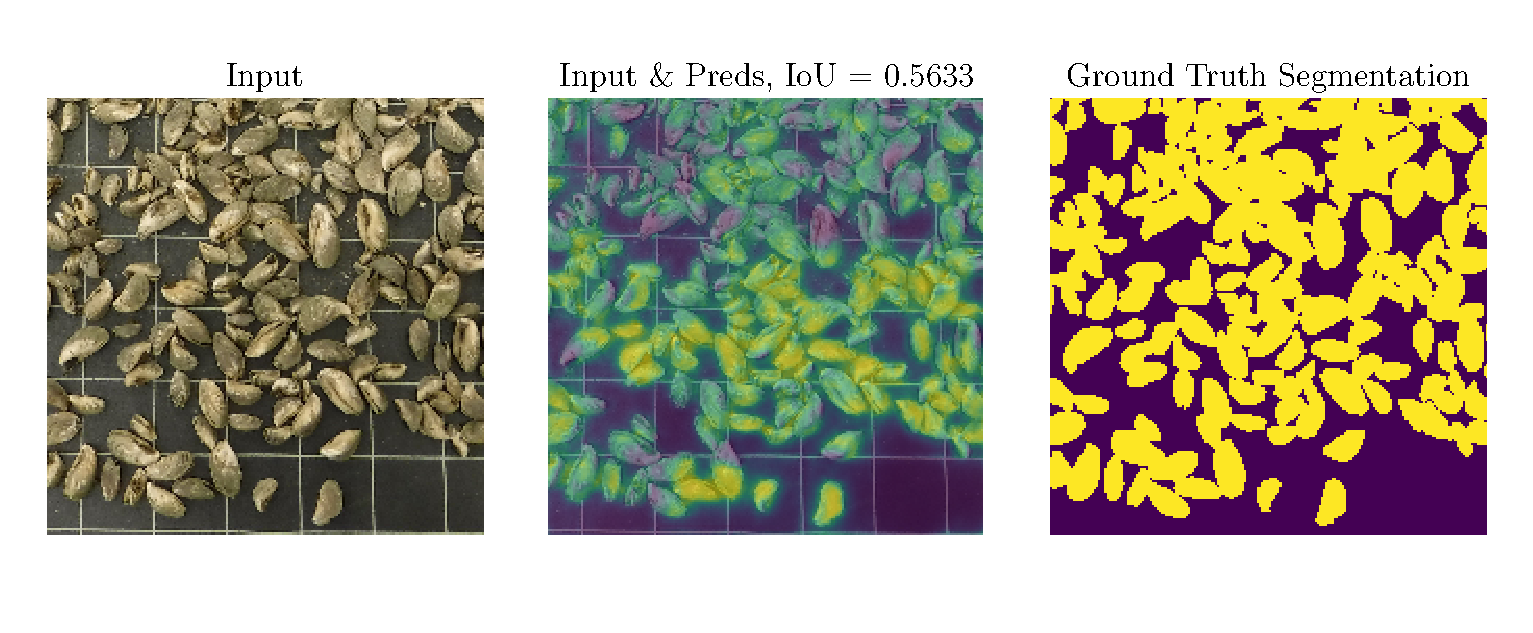
\includegraphics[width=0.9\linewidth]{\zshot/val_101-lab_100__Lab_3801-1_2018-07-11_image-1_patch_width1200__fcn8s_lr1e-03_wd5e-04_bs25_ep80_seed4_epoch70.eps}}

\caption{Qualitative results and intersection-over-union (IoU) score arising
from training the~\texttt{FCN8s} model on~\emph{in situ} underwater data
(\texttt{val\_v101} split -- ``in distribution'') and testing on Lab data 
(\texttt{v100} -- ``out of distribution''), a.k.a ``zero-shot'' generalization. 
The first column is an input patch in RGB format, second column 
overlays the real valued sigmoid prediction score with the input, and the last 
row are the ground truth binary masks. A failure case is shown in the first
row, and more successful cases in other rows. See text for more details. 
Note: predictions are binarized for calculating IoU. All images are $1200$
square pixels for clarity.}
\label{fig:zero-shot-situ-lab}
\end{figure}


\subsection{Predicting Live Mussel Count}

The labels in the lab analysis for all $N=40$ images from the 2019 Lab test 
split were used to characterize the irreducible error between 
the~\texttt{Count} and~\texttt{Biomass} variables. This serves as a key
baseline before attempting to predict live mussel count using DL. 
Figure~\ref{fig:count-from-biomass} depicts this relationship before and after 
correcting biomass by the mussel size distribution variable. 

For sample index $i$, a size distribution vector $\gamma \in \mathbb{R}^8$ with 
elements $j$ being the fraction of mussels not passing the $X_j$ mm sieve, 
$X \in \{16, 14, 12.5, 10, 8, 6.3, 4, 2\}$, the biomass $\text{B}_i$ was 
adjusted according to:

\begin{equation} \label{eq:size-distribution}
\text{Count}_i = \text{B}_i \cdot \Sigma_{j=1}^8 \bigg( \gamma_j \cdot \frac{2 
\text{mm}}{X_j} \bigg)
\end{equation}

The constant 2 mm in the numerator of Eq.~\eqref{eq:size-distribution} is the 
minimum sieve size, such that biomass associated with this bin contributes 
$1:1$ to the mussel Count, while the weight associated with biomass belonging 
to larger mussels decreases with the ratio of the diameter to the smallest 2 mm
diameter.

\begin{figure}
\centering
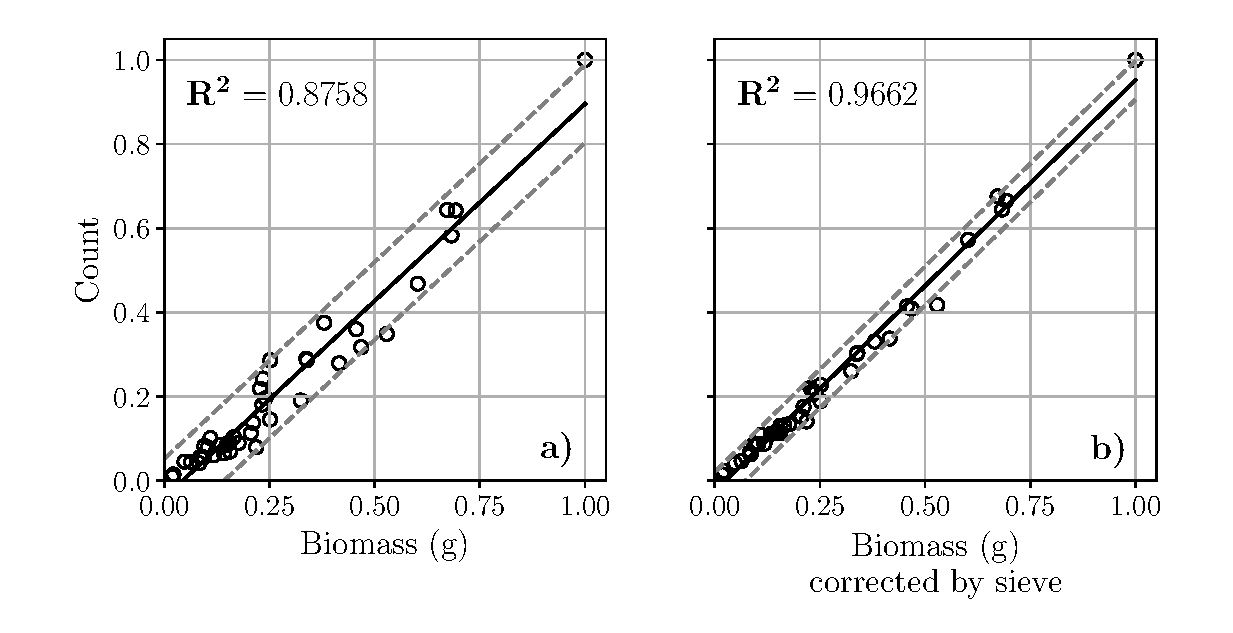
\includegraphics[width=0.9\linewidth]{img/lab_count_from_biomass.eps}
\caption{The relationship between live mussel count and biomass (grams)
for all $N=40$ samples from the 2019~\texttt{Lab} dataset, (a) before, and (b) 
after correcting for the size distribution using
Eq.~\eqref{eq:size-distribution}. The dashed lines indicate two standard
deviations from the line of best fit.}
\label{fig:count-from-biomass}
\end{figure}

\begin{figure}
\centering
\includegraphics[width=0.9\linewidth]{img/lab_predict_count_val_100-val_100__fcn8slim_lr1e-03_wd5e-04_bs32_ep50_seed1_epoch40.eps}
\caption{Prediction of live mussel count for $N=38$ samples (two outliers were
removed, see text for details) from the 2019~\texttt{Lab} dataset, (a) before, 
and (b) after camera adjustment. Prediction is based on watershed segmentation 
of the prediction mask. The dashed lines indicate two standard deviations from
the line of best fit.}
\label{fig:count-from-watershed}
\end{figure}

\begin{figure}
\centering
\subfigure[]{
\includegraphics[width=0.4\linewidth]{img/Lab_3554-1_2018-07-04_image-1_watershed_actual_count21_pcount16.png}
\label{sub:watershed-3554-1}}
\subfigure[]{
\includegraphics[width=0.4\linewidth]{img/Lab_3796-1_2018-08-13_image-1_watershed_actual_count122_pcount43.png}
\label{sub:watershed-3796-1}}
\caption{Two examples of watershed segmentation results for counting live
mussels in the 2019~\texttt{Lab} dataset. Each colour denotes a unique mussel
instance. 
In~\subref{sub:watershed-3554-1}, 21 total mussels were reported in 
the lab analysis, of which 16 are identified. The six mussels that were 
missed are the six smallest in diameter. It was found that the distance 
thresholds in the watersheed algorithm could be tuned to recover some of the 
smaller mussels, but there was a trade-off in terms of the type of error we see 
in~\subref{sub:watershed-3796-1} where some mussels that were touching could 
not be separated.}
\label{fig:watershed-samples}
\end{figure}

\iffalse
\begin{figure}
\centering
\includegraphics[width=\linewidth]{./img/trainval_111-Tripod__Lab_1352_2019-05-23_GoPro-1__fcn8s_lr1e-03_wd5e-04_bs40_ep80_seed2amp_epoch79_iou_0p4103.jpg}
\caption{Zero-shot generalization from~\texttt{trainval\_v111} split to Tripod
site 1352, still image from May 23, with an IoU of 0.4103 with the ground truth 
mask. Note that there are some false positives on the chain link, but this is 
reasonable as the object was not encountered during training, and forms a 
curved edge with shadow similar to that of a mussel.}
\label{fig:tripod-1352}
\end{figure}
\fi


\section{Conclusion and Recommendations}

The following recommendations are optional, and may be adopted independently of 
the other recommendations or simultaneously. Adopting any of these changes 
should increase the accuracy with which biomass and population counts can be 
estimated.

\begin{description}
	
	\item[Crowdsource Additional High Quality Labels] It is anticipated that 
	performance in terms of both prediction IoU and lab measurements could be 
	further improved by seeking additional labels. Based on the comparison
	outlined in Table~\ref{tab:label-services}, the most suitable service in 
	light of estimated volume and label quality is Scale, which charges a flat 
	\$6.40 USD fee per label. This is a relatively inexpensive and guaranteed
	way to improve model performance.
	
	\item[Illumination]	It was observed that some images use artificial 
	lighting while many do not. It would be helpful to standardize this, 
	ideally using the additional light unless the scene is already well lit.
	
	\item[Distance from Camera to Bottom] The camera to object distance should 
	be as consistent as possible.
	
	\item[Occlusion] Vegetation should be removed
	
	\item[Seasonal Changes] It is known that Cladophora and other green algae 
	grow as the summer season progresses. As an alternative to manual removal 
	of debris from the area of interest, the collection of training data and 
	model deployment could be coordinated around a specific time interval each 
	year, for example May and June when algae is less present.
	
	\item[Ambiguous Shells] Empty shells pose a challenge both for labeling and 
	the models. Although models showed a good ability to distinguish the mostly
	darker Zebra mussels from white shells, the Quagga mussel can be lighter in 
	colour than the Zebra and hard to discriminate from the spurious shells 
	during labeling. Depending on the orientation of the shell, if the exterior
	is facing up it it impossible to determine if it is ``dead'', or contains a
	second shell piece underneath and is a live animal. 
	
	Rather than interpreting the categorical~\texttt{mussel} label to include
	Zebra and Quagga mussels and not white shells, it would be helpful to 
	standardize around the shell colour, and for example use separate classes 
	for dark versus white shells, or try to capture images in areas with few 
	empty shells and include them in the~\texttt{mussel} class. 
	Alternatively, empty shells could be removed but this requires manual 
	intervention.
	
\end{description}


\clearpage

%\bibliographystyle{spbasic} % basic style, author-year citations
\bibliography{CCIW_Zebra}   % name your BibTeX data base

\clearpage

\appendix

\section{Data Annotation Services}

\subsection{Figure Eight}
\label{sec:figure-eight}

Additional settings were required for good results with this platform. 
Under the Design tab, at the bottom of the page there is an option to enable 
the Code Editor. A new field ``CML'' appears in the editor, which was modified 
as follows:

\begin{lstlisting}[language=html, frame=single]
<cml:shapes label="Draw Shapes" name="annotation" 
type="['polygon']" image-url="{{image_url}}" 
polygon-threshold="0.15" class-threshold="0.1" 
ontology="true" crosshair="false" validates="required" 
class-agg="cagg_0.1" polygon-agg="0.1" gold="true"/>
\end{lstlisting}

The variables modified were: 

\begin{description}
\item[polygon-threshold] The minimum time it should take a contributor to
complete a page of work. When triggered, the contributor will be removed from
your job. Increased from default of 10 to 20 seconds.
\end{description}

These variables are documented here:\url{ 
https://success.figure-eight.com/hc/en-us/articles/360016693051-Guide-to-Polygon-Job-Design-Test-Questions-and-Aggregation}

Under Settings $>$ Contributors:

Increased the ``contributor level'' from level 1 -- \textbf{Fastest
Throughput}: All qualified contributors, to level 3 -- highest quality: 

Under Settings $>$ Quality Control:

\begin{description}
\item[Minimum Time Per Page] The minimum time it should take a contributor to
complete a page of work. When triggered, the contributor will be removed from
your job. Increased from default of 10 to 20 seconds.

\item[Results] check the box to disable responses to test questions.
\end{description}

Post processing json output from FigureEight for validation in LabelMe. We need 
to convert the report generated by FigureEight, which is in jsonstring format, 
into plain json. 

\begin{lstlisting}[language=bash, frame=single]
sed '1s/^/[/; $!s/$/,/; $s/$/]/' in.json > out.json

1  s/^/[/      # Insert a left bracket at the beginning of the first line
$! s/$/,/      # On all but the last line append a comma
$  s/$/]/      # Append a right bracket to the last line
\end{lstlisting}

\subsection{Scale AI}

This section enumerates the complete set of steps to process the output of the 
Scale AI platform for use by the python model training scripts.

\begin{enumerate}

\item Request labels from Scale using Listing~\ref{lst:scale}, 
where~\texttt{csv\_file} is a list of files available at a public URL 
like:\\
\texttt{https://<bucket>.amazonaws.com/<path>/GLNI\_PSN-Quad\_YYYY-MM-DD\_image-\#.jpg}

\begin{lstlisting}[language=python, caption=A complete Python snippet for 
requesting semantic segmentation labels from the Scale annotation service
for an arbitrary number of images specified in~\texttt{csv\_file}., 
frame=single, label={lst:scale}]
import scaleapi
client = scaleapi.ScaleClient(API_KEY)  # API_KEY from scale.com
with open(os.path.join(csv_path, csv_file)) as f:
  csv_reader = csv.reader(f, delimiter=',')
  for row in csv_reader:
    resp = client.create_segmentannotation_task(
      urgency='standard',  # optional: immediate
      callback_url='your@email.com',
      instruction='Draw a tight polygon around the live **mussels**
        in the image. Ignore empty white shells.',
      attachment_type='image',
      attachment=row[0],
      labels=['background', 'mussel'],
      allow_unlabeled=False
    )
\end{lstlisting}    

\item Run the python
notebook~\href{https://github.com/AngusG/cciw-zebra-mussel/blob/master/labelme/scale}{postprocess-scale-labels.ipynb}
to convert the RGB colour labels from the~\texttt{Scale AI} API into the format
consistent with the~\texttt{labels.txt} file used by~\texttt{LabelMe}.

\item Run the python
notebook~\href{https://github.com/AngusG/cciw-zebra-mussel/blob/master/labelme/voc-images-and-masks-to-patch.ipynb}{voc-images-and-masks-to-patch.ipynb}
to extract small patches from each labeled image and mask for training and
validation.

\item Populate the test.txt file for VOC format:

\begin{lstlisting}[language=bash, frame=single]
user@ws1:~/Dataset/Test/GLNI/port/scale/patches$ 
ls -l *.png >> VOCdevkit/VOC2012/ImageSets/Segmentation/test.txt
\end{lstlisting}

\item Copy masks into the relevant VOCdevkit folder:

\begin{lstlisting}[language=bash, frame=single]
user@ws1:~/Dataset/Test/GLNI/port/scale/patches$ 
cp -av *.png VOCdevkit/VOC2012/SegmentationClass/
\end{lstlisting}

\item Copy jpeg images into the relevant VOCdevkit folder:

\begin{lstlisting}[language=bash, frame=single]
user@ws1:~/Dataset/Test/GLNI/port/scale/patches$ 
cp -av *.jpg VOCdevkit/VOC2012/JPEGImages/
\end{lstlisting}

\item Confirm that each folder contains the same number of images:
\begin{lstlisting}[language=bash, frame=single]
ls -l VOCdevkit/VOC2012/SegmentationClass | wc -l
ls -l VOCdevkit/VOC2012/JPEGImages/ | wc -l
\end{lstlisting}

\end{enumerate}

\subsection{Editing Segmentation Masks in GIMP}
\label{sec:gimp}

This section outlines a procedure for editing segmentations masks in PNG format
rather than as~\texttt{json} vertices, for example to clean up the
automatically generated masks for the Lab images from the
notebook~\href{https://github.com/AngusG/cciw-zebra-mussel/blob/master/labelme/autolabel-lab-testing-set.ipynb}{autolabel-lab-testing-set.ipynb},
 or those returned by the~\url{https://scale.com/} service.

I recommend using the~\href{https://www.gimp.org/}{GNU Image Manipulation
Program} (GIMP), which is a free and open source professional graphics software 
program, albeit with a bit of a learning curve.

\begin{enumerate}
\item Select a~\texttt{*.jpg} image, right click and open with GIMP Image 
Editor.
\item In the Layers pane, select this jpg layer and click on the paint brush 
icon ``Lock pixels'' to freeze this layer.
\item From the main menu, select File, Open as Layers..., and select the PNG 
mask associated for the image.
\item Select the PNG mask from the layers pane and change the Opacity value
from $100\%$ to $50\%$.

\item To efficiently label data, I made use of the ``Free Select Tool'' from
the Toolbox, which can be enabled with the keyboard shortcut ``f''. I then fill
in the polygon drawn with the Free Select Tool using the ``Bucket Fill Tool''. 
The Bucket Fill tool default shortcut is ``Shift B'', which can be cumbersome 
when switching rapidly back and fourth. I created a new shortcut ``b'' using 
the instructions 
here:~\url{https://docs.gimp.org/2.10/en/gimp-concepts-shortcuts.html}.

\item Change the foreground color to solid red (\texttt{\#ff0000}), consistent
with the existing indexed colormap of the mussel labels, but a bit brighter to
make it easier to see which pixels have been changed in GIMP. The
notebook~\texttt{run-crf-on-gimp-masks.ipynb} ultimately merges the two red
variants into a single ``mussel'' label. Change the background color to 
black (\texttt{\#000000}). We will use this to remove any ``false positives'', 
that is, pixels predicted as mussel that should be background.

\item Under Bucket Fill, Tool Options, change ``Affected Area'' to ``Fill whole 
selection''.

\item Use the shorcut ``f'' to enable the Free Select Tool and draw the first 
polygon around a mussel. Note that you may either click to place individual
vertices, or press and hold the left mouse to draw a continous curve. Next, use
the ``b'' or ``Shift+B'' shortcut to switch to Bucket Fill. Ensure ``FG color
fill'' is selected which will use the red colour set previously for mussel. 
Similarly, to label background pixels, switch the Fill Type to ``BG color 
fill''. Repeat this step as necessary until satisfied.

\begin{figure}
\centering
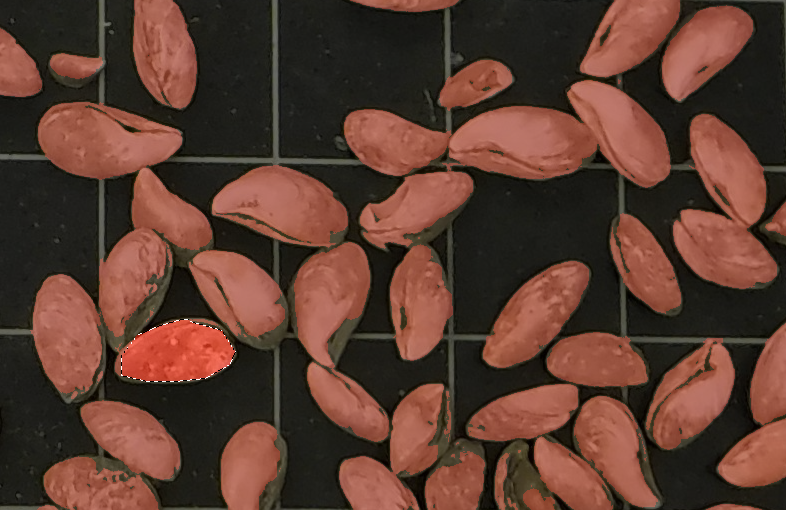
\includegraphics[width=0.4\linewidth]{img/GIMP_edit_mask}
\caption{Modifying mussel segmentation masks using GIMP software. Transparent 
red colour corresponds to mussel label. Selected area corresponds to modified 
label.}
\label{fig:gimp-label}
\end{figure}

\item To export a new mask in the correct format, we will now delete the JPEG 
layer. From the Layers pane, right click on the jpg file and select ``Delete
Layer''. Now select the PNG layer that we have been editing, and restore the 
Opacity to $100\%$. 

\item Select Image $\rightarrow$ Mode $\rightarrow$ Indexed from the 
main menu to change the image from RGB format to indexed color 
format. The default setting, choose optimal colormap can be 
used. For more information 
see~\url{https://docs.gimp.org/2.8/en/gimp-image-convert-indexed.html}.

\item Finally, from the File menu, Export As and append~\texttt{\_gimp.png} to 
the end of the file for reproducibility. Each Lab sample should now be 
associated with the following collection of five (5) images:

\begin{figure}
\centering
\subfigure[]{
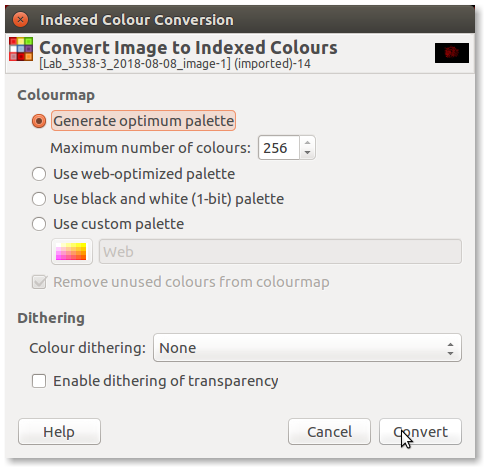
\includegraphics[width=0.4\linewidth]{img/GIMP_Indexed-color-conversion}}
\subfigure[]{
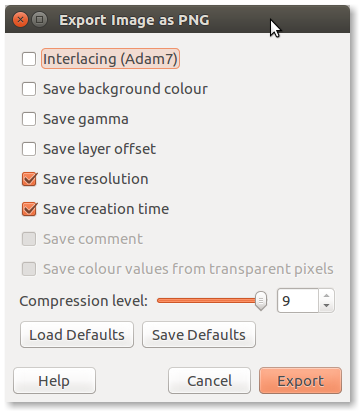
\includegraphics[width=0.34\linewidth]{img/GIMP_Export-Image-as-PNG}}
\caption{gimp-usage}
\label{fig:gimp-export-menu}
\end{figure}

\begin{enumerate}
\item \texttt{Lab\_2907-3\_2018-07-09\_image-1.jpg} -- Original RGB JPEG image.
\item \texttt{Lab\_2907-3\_2018-07-09\_image-1\_mask\_crf.png} -- Indexed color 
PNG mask, noisy output from~\texttt{autolabel-lab-testing-set.ipynb}.
\item \texttt{Lab\_2907-3\_2018-07-09\_image-1\_mask\_crf.xcf} -- GIMP version 
of file (b) for editing.
\item \texttt{Lab\_2907-3\_2018-07-09\_image-1\_mask\_crf\_gimp.png} -- Updated 
indexed color PNG mask after processing in GIMP. Contains two shades of red, 
GIMP changes in bright red.
\item \texttt{Lab\_2907-3\_2018-07-09\_image-1\_mask\_crf\_gimp\_crf.png} -- 
After processing of file (d) with~\texttt{run-crf-on-gimp-masks.ipynb}. Contains
only a single label index, suitable for use with Python DL model training and
testing scripts.

\end{enumerate}

\end{enumerate}

\end{document}
